\clearpage
%//==============================--@--==============================//%
\subsection[2.3 Reguladores de tensão]{\hspace*{0.075 em}\raisebox{0.2 em}{$\pmb{\drsh}$} Reguladores de tensão}
\label{subsec:reguladores-tensao}

\begin{figure}[H]
    \centering
    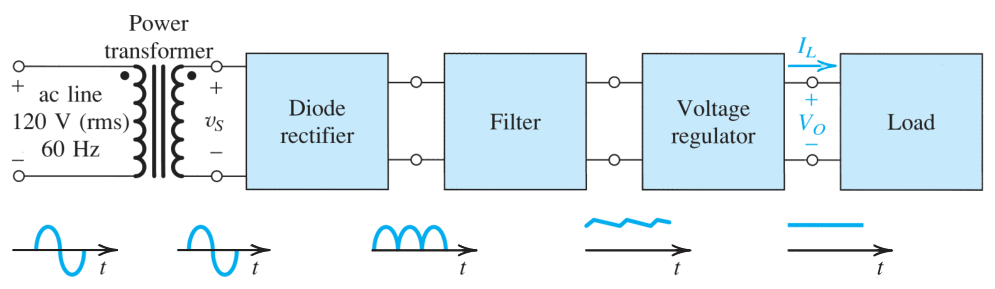
\includegraphics[width=0.8\linewidth]{img/2/power-supply-block-diagram.png}
    \caption{Exemplo com aplicações de díodos. ``Block diagram of a DC power supply.''\cite{sedra-smith:microelectronic-circuits}}
    \label{fig:power-supply-block-diagram}
\end{figure}

\renewcommand*{\thefootnote}{\fnsymbol{footnote}}
\footnotetext[4]{%
    ``Nas fontes de alimentação usa-se, normalmente, um transformador, de modo a baixar a amplitude da tensão alternada e, consequentemente, o valor da tensão continua produzida. Isto é necessário porque a tensão da rede tem amplitude elevada ($220 \sqrt{2} = 311$V) e as tensões contínuas para alimentação dos circuitos electrónicos são muito menores (por exemplo, $12$V). O transformador tem, além disso, a vantagem de produzir \textbf{isolamento galvânico} em relação à rede (há apenas ligação magnética entre os enrolamentos do transformador), o que é útil do ponto de vista da segurança.''\cite{medeiros:ICEE}
}
\renewcommand*{\thefootnote}{\arabic{footnote}}

\noindent Uma \textbf{fonte de tensão} tem como objetivo produzir uma tensão $v_O$ constante. Para tal, necessita, após do retificador e do filtro RC previamente discutido, de um \textbf{regulador de tensão} com vista a \textbf{reduzir o tremor}:

\begin{figure}[H]
    \centering
    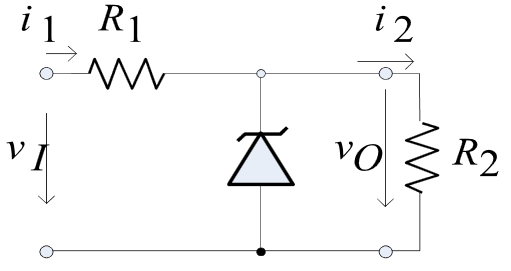
\includegraphics[width = 0.4\linewidth]{img/2/reg-ten.png}
    \caption{Regulador de tensão}
    \label{fig:reg-tensão}
\end{figure}

\begin{quote}
    ``\textbf{Zener Diodes} can be used to produce a \underline{stabilised voltage output} with low ripple under varying load current conditions. By passing a small current through the diode from a voltage source, via a suitable \underline{current limiting resistor} ($R_1$), the zener diode will conduct sufficient current to maintain a voltage drop of $V_\textit{out}$."
\end{quote}

\vspace{0.7 em}
\begin{center}
    \begin{minipage}{0.6\textwidth}
        \begin{itemize}[leftmargin=*]
        \item[] Supondo o díodo em corte:
        $$
            \boxed{v_O = \dfrac{R_2}{R_1 + R_2}v_I}
        $$

        Quando $v_O$ (que se encontra dependente de $v_I$) ultrapassa o treshold $V_Z$ (isto é, $v_I > V_Z$), a tensão na \textit{load} é limitada a $V_Z$. 
        
        Quando $v_O > V_Z$ o díodo entra em condução:
        $$
            \boxed{v_O = V_Z}
        $$
        \end{itemize}
    \end{minipage}%
    \hfill
    \begin{minipage}{0.4\textwidth}
        \begin{center}
            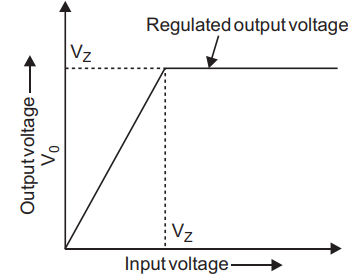
\includegraphics[width=0.9\textwidth]{img/2/chara-ten-reg.png}
            \label{img:chara-ten-reg}
        \end{center}
    \end{minipage}
\end{center}
\noindent \textbf{Nota:} Usa-se para potências muito baixas, de forma a que $i_2 \simeq 0$
%//==============================--@--==============================//%